\documentclass[12pt]{article}

%------------- PREAMBLE -------------
\usepackage[margin=1in]{geometry}
\usepackage{amsmath,amssymb,mathtools}
\usepackage{enumitem}
\usepackage{bm}
\usepackage{hyperref}
\usepackage{fancyhdr}
\usepackage{draftwatermark}
\usepackage{xcolor}
\usepackage{titlesec}
\usepackage{tikz}
\usetikzlibrary{arrows.meta,calc,positioning}

%------------- TITLE AND METADATA -------------
\newcommand{\CourseCode}{MH1301}
\newcommand{\CourseName}{Discrete Mathematics}
\newcommand{\DocType}{Tutorial 11}

\title{
\CourseCode\ \CourseName \\[0.3em]
\large \DocType
}
\author{
  Academic Year 2025/2026, Semester 2 \\[0.25em]
  \textit{Quantitative Research Society @NTU}
}
\date{\today}

%------------- HEADER & FOOTER (for page 2 onward) -------------
\fancypagestyle{main}{
  \fancyhf{}
  \fancyhead[L]{\CourseCode\ \CourseName}
  \fancyhead[R]{\href{https://qrsntu.org}{QRS@NTU}}
  \fancyfoot[C]{\thepage}
  \renewcommand{\headrulewidth}{0.4pt}
  \renewcommand{\footrulewidth}{0pt}
}

%------------- SIMPLE FOOTER (page 1 only) -------------
\fancypagestyle{plainfirst}{
  \fancyhf{}
  \renewcommand{\headrulewidth}{0pt}
  \renewcommand{\footrulewidth}{0pt}
  \fancyfoot[C]{\scriptsize\textcolor{gray}{\textit{For academic reference only. This document is provided for educational purposes and does not constitute an official question paper, answer key, or any formally authorised academic material. Its content is not guaranteed to be complete or accurate.}}}
}

%------------- WATERMARK -------------
\SetWatermarkText{Unofficial --- QRS@NTU --- qrsntu.org}
\SetWatermarkScale{1}
\SetWatermarkLightness{0.985}

%------------- SHORTCUTS -------------
\newcommand{\N}{\mathbb{N}}
\newcommand{\Z}{\mathbb{Z}}
\newcommand{\R}{\mathbb{R}}
\newcommand{\comp}[1]{\overline{#1}}
\newcommand{\V}{V}
\newcommand{\E}{E}
\newcommand{\degG}{\deg}
\newcommand{\diam}{\operatorname{diam}}

\DeclareMathOperator{\dist}{dist}

\tikzset{
  vtx/.style={circle, draw, minimum size=20pt, inner sep=1pt},
  dotv/.style={circle, fill, inner sep=1.5pt},
  smallv/.style={circle, fill, inner sep=1.1pt},
  every picture/.style={line cap=round, line join=round}
}

\setcounter{secnumdepth}{-1}
\setcounter{tocdepth}{3}
\setlist[enumerate]{itemsep=0.3em, topsep=0.3em}
\setlist[itemize]{itemsep=0.2em, topsep=0.2em}
\setlength{\headheight}{14.5pt}

\begin{document}

%------------- COVER PAGE -------------
\maketitle
\thispagestyle{plainfirst}
\pagestyle{main}

%====================================================
% OVERVIEW
%====================================================
\begin{center}
  \rule{0.82\textwidth}{0.4pt}\\[4pt]
  \textbf{Overview}\\[2pt]
  \rule{0.82\textwidth}{0.4pt}
\end{center}

\noindent
This tutorial develops the basic theory of trees, forests, complete bipartite trees, and binary trees. The main themes are:
\begin{itemize}[leftmargin=*]
  \item classification of trees with a vertex of very large degree;
  \item equivalent characterisations of trees using connectivity, cycles, and bridges;
  \item identifying which complete bipartite graphs are trees;
  \item edge-count formulae for trees, forests, and full binary trees;
  \item construction and counting formulae for complete binary trees.
\end{itemize}

\noindent
\textbf{Question map.}
\begin{itemize}[leftmargin=*]
  \item Questions 1--3: non-isomorphic trees with one vertex of degree $n-1$, $n-2$, or $n-3$.
  \item Question 4: a bridge-deletion characterisation of trees.
  \item Question 5: complete bipartite graphs that are trees.
  \item Questions 6--7: edge counts in trees, full binary trees, and forests.
  \item Question 8: complete binary trees of height $h$.
\end{itemize}

\newpage
\tableofcontents

%====================================================
% QUESTION 1
%====================================================
\newpage
\section{Question 1 (Trees with a vertex of degree $n-1$)}

\subsection{Problem}
Assume that $n\ge 7$. How many non-isomorphic trees with $n$ vertices are there in which one vertex has degree $n-1$?

\subsection{Solution}

\subsubsection{Method 1: Direct degree-neighbourhood classification}
Let $T$ be a tree on $n$ vertices. Suppose some vertex $v\in V(T)$ has
\[
  \deg(v)=n-1.
\]
Since $T$ has exactly $n$ vertices, the vertex $v$ is adjacent to every other vertex.

Thus every edge incident with $v$ is of the form
\[
  vv_i,
  \qquad
  v_i\in V(T)\setminus\{v\}.
\]
There are already $n-1$ such edges. A tree on $n$ vertices has exactly $n-1$ edges, so there can be no further edges among the vertices in $V(T)\setminus\{v\}$.

Therefore
\[
  T\cong K_{1,n-1},
\]
the star on $n$ vertices. Hence there is exactly one isomorphism type:
\[
  \boxed{1}.
\]

\subsubsection{Method 2: Edge-count extremal argument}
\textbf{Theorem/criterion used.} Every tree on $n$ vertices has exactly $n-1$ edges.

If a vertex $v$ has degree $n-1$, then the edges incident with $v$ already account for
\[
  n-1
\]
distinct edges. Since a tree on $n$ vertices has exactly $n-1$ edges, these are all the edges of the tree.

Hence the tree is completely determined:
\[
  E(T)=\{vv_i: v_i\in V(T)\setminus\{v\}\}.
\]
This is the star $K_{1,n-1}$. Therefore all such trees are isomorphic, and the number of non-isomorphic trees is
\[
  \boxed{1}.
\]

%====================================================
% QUESTION 2
%====================================================
\newpage
\section{Question 2 (Trees with a vertex of degree $n-2$)}

\subsection{Problem}
Assume that $n\ge 7$. How many non-isomorphic trees with $n$ vertices are there in which one vertex has degree $n-2$?

\subsection{Solution}

\subsubsection{Method 1: Edge-budget classification}
Let $T$ be a tree on $n$ vertices. Suppose some vertex $v$ has
\[
  \deg(v)=n-2.
\]
Then $v$ is adjacent to exactly $n-2$ of the other $n-1$ vertices. Hence there is exactly one vertex, say $x$, not adjacent to $v$.

The $n-2$ edges incident with $v$ already occur in $T$. Since $T$ has exactly $n-1$ edges, there is exactly one remaining edge. The vertex $x$ must be connected to the rest of the graph because $T$ is connected. Since $x$ is not adjacent to $v$, this remaining edge must connect $x$ to one of the neighbours of $v$.

All neighbours of $v$ are symmetric under isomorphism. Therefore every such tree is isomorphic to a star with one pendant edge subdivided once:
\begin{center}
\begin{tikzpicture}[scale=1.0]
  \node[dotv,label=above:$v$] (v) at (0,1.5) {};
  \node[dotv] (a) at (-2,0) {};
  \node[dotv] (b) at (-0.7,0) {};
  \node[dotv] (c) at (0.7,0) {};
  \node[dotv] (d) at (2,0) {};
  \node[dotv,label=below:$x$] (x) at (-2,-1.2) {};
  \draw (v)--(a)--(x);
  \draw (v)--(b);
  \draw (v)--(c);
  \draw (v)--(d);
  \node at (1.35,-0.12) {$\cdots$};
\end{tikzpicture}
\end{center}
Thus there is exactly one non-isomorphic tree of this type:
\[
  \boxed{1}.
\]

\subsubsection{Method 2: Branch-length partition}
Root the tree at the vertex $v$ of degree $n-2$. Since $v$ has $n-2$ incident edges, it has $n-2$ branches starting from it.

There are
\[
  n-1
\]
vertices other than $v$. These are distributed among $n-2$ branches. Each branch contains at least one vertex. Hence the branch-size multiset is a partition of $n-1$ into $n-2$ positive parts:
\[
  n-1=2+1+\cdots+1.
\]
Thus exactly one branch has length $2$, and all other branches have length $1$. This determines the rooted tree up to isomorphism, and hence determines the unrooted tree up to isomorphism.

Therefore the number of non-isomorphic trees is
\[
  \boxed{1}.
\]

%====================================================
% QUESTION 3
%====================================================
\newpage
\section{Question 3 (Trees with a vertex of degree $n-3$)}

\subsection{Problem}
Assume that $n\ge 7$. How many non-isomorphic trees with $n$ vertices are there in which one vertex has degree $n-3$?

\subsection{Solution}

\subsubsection{Method 1: Component classification after deleting the high-degree vertex}
Let $T$ be a tree on $n$ vertices. Suppose some vertex $v$ has
\[
  \deg(v)=n-3.
\]
Deleting $v$ from a tree separates the tree into exactly $\deg(v)$ components. Therefore
\[
  T-v
\]
is a forest with
\[
  n-1
\]
vertices and
\[
  n-3
\]
components.

A forest with $N$ vertices and $c$ components has $N-c$ edges. Hence
\[
  |E(T-v)|=(n-1)-(n-3)=2.
\]
Thus the classification reduces to classifying a forest on $n-1$ vertices with exactly $2$ edges and $n-3$ components, where the $n-3$ components correspond to the $n-3$ branches from $v$.

There are exactly three possible component types involving the two additional edges:
\[
  K_2\sqcup K_2,\qquad K_{1,2},\qquad P_3.
\]
Equivalently, the tree has one of the following three branch patterns at $v$:
\[
\begin{array}{c@{\qquad}c@{\qquad}c}
\text{A: two branches of length }2
&
\text{B: one split branch}
&
\text{C: one branch of length }3
\end{array}
\]

\begin{center}
\begin{tikzpicture}[scale=0.95]
  % Type A
  \begin{scope}[shift={(-5.0,0)}]
    \node[dotv,label=above:$v$] (v) at (0,1.6) {};
    \node[dotv] (a) at (-1.2,0.2) {};
    \node[dotv] (b) at (0,0.2) {};
    \node[dotv] (c) at (1.2,0.2) {};
    \node[dotv] (aa) at (-1.2,-1.0) {};
    \node[dotv] (bb) at (0,-1.0) {};
    \draw (v)--(a)--(aa);
    \draw (v)--(b)--(bb);
    \draw (v)--(c);
    \node at (0.62,0.02) {$\cdots$};
    \node at (0,-1.65) {A};
  \end{scope}

  % Type B
  \begin{scope}[shift={(0,0)}]
    \node[dotv,label=above:$v$] (v) at (0,1.6) {};
    \node[dotv] (a) at (-1.2,0.2) {};
    \node[dotv] (b) at (0.2,0.2) {};
    \node[dotv] (c) at (1.3,0.2) {};
    \node[dotv] (aa) at (-1.8,-1.0) {};
    \node[dotv] (ab) at (-0.6,-1.0) {};
    \draw (v)--(a);
    \draw (a)--(aa);
    \draw (a)--(ab);
    \draw (v)--(b);
    \draw (v)--(c);
    \node at (0.78,0.02) {$\cdots$};
    \node at (0,-1.65) {B};
  \end{scope}

  % Type C
  \begin{scope}[shift={(5.0,0)}]
    \node[dotv,label=above:$v$] (v) at (0,1.6) {};
    \node[dotv] (a) at (-1.2,0.2) {};
    \node[dotv] (b) at (0,0.2) {};
    \node[dotv] (c) at (1.2,0.2) {};
    \node[dotv] (aa) at (-1.2,-0.9) {};
    \node[dotv] (aaa) at (-1.2,-2.0) {};
    \draw (v)--(a)--(aa)--(aaa);
    \draw (v)--(b);
    \draw (v)--(c);
    \node at (0.62,0.02) {$\cdots$};
    \node at (0,-2.55) {C};
  \end{scope}
\end{tikzpicture}
\end{center}

These three types are pairwise non-isomorphic:
\begin{itemize}[leftmargin=*]
  \item Type A has two vertices at distance $2$ from $v$ and none at distance $3$ from $v$.
  \item Type B has a neighbour of $v$ of degree $3$.
  \item Type C has one vertex at distance $3$ from $v$.
\end{itemize}
Thus there are exactly three non-isomorphic trees:
\[
  \boxed{3}.
\]

\subsubsection{Method 2: Branch-size partitions and branch shapes}
Root the tree at a vertex $v$ of degree $n-3$. Then there are $n-3$ branches from $v$, and these branches contain all
\[
  n-1
\]
vertices other than $v$.

Thus the branch sizes form a partition of $n-1$ into $n-3$ positive integers. Equivalently, starting from
\[
  1+1+\cdots+1
\]
with $n-3$ parts, we must distribute two additional vertices among the branches. There are two possible size patterns:
\[
  3,1,1,\dots,1
  \qquad\text{or}\qquad
  2,2,1,\dots,1.
\]

For the pattern
\[
  2,2,1,\dots,1,
\]
both branches of size $2$ are forced to be paths of length $2$. This gives Type A.

For the pattern
\[
  3,1,1,\dots,1,
\]
there are two rooted tree shapes on a branch of size $3$:
\[
  \text{a path of length }3
  \qquad\text{or}\qquad
  \text{one neighbour with two children}.
\]
These give Type C and Type B respectively.

Hence the total number of rooted branch shapes, and therefore the total number of non-isomorphic unrooted trees, is
\[
  1+2=3.
\]
Therefore
\[
  \boxed{3}.
\]

%====================================================
% QUESTION 4
%====================================================
\newpage
\section{Question 4 (Bridge-deletion characterisation of trees)}

\subsection{Problem}
\textbf{(Ex 11.1.8).} Prove that a simple graph is a tree if and only if it is connected, but the deletion of any of its edges produces a graph that is not connected.

\subsection{Solution}

\subsubsection{Method 1: Cycle contradiction and bridge property}
\textbf{Theorem/criterion used.} A tree is a connected simple graph with no circuits. An edge is a bridge if deleting it disconnects the graph.

We prove both directions.

\medskip
\noindent
\textbf{Forward direction.} Suppose $G$ is a tree. Let $e=uv\in E(G)$. Consider $G-e$.

If $G-e$ were connected, then there would still be a path from $u$ to $v$ in $G-e$. Let this path be
\[
  u=x_0,x_1,\dots,x_k=v.
\]
Then in $G$, the path together with the edge $uv$ forms a circuit:
\[
  u=x_0,x_1,\dots,x_k=v,u.
\]
This contradicts the fact that a tree has no circuits. Hence $G-e$ is disconnected. Since $e$ was arbitrary, deleting any edge of $G$ disconnects the graph.

\medskip
\noindent
\textbf{Reverse direction.} Suppose $G$ is connected and deleting any edge disconnects $G$. We prove that $G$ has no circuit.

Assume for contradiction that $G$ contains a circuit
\[
  C=v_1v_2\cdots v_kv_1.
\]
Delete the edge
\[
  e=v_1v_2.
\]
The vertices $v_1$ and $v_2$ remain connected in $G-e$ by the path
\[
  v_1,v_k,v_{k-1},\dots,v_2.
\]
Moreover, any path in $G$ that used the deleted edge $v_1v_2$ can replace that edge by the remaining part of the circuit. Thus deleting $e$ does not disconnect $G$, contradicting the hypothesis.

Therefore $G$ is connected and has no circuit. Hence $G$ is a tree.

Thus
\[
  \boxed{G\text{ is a tree if and only if }G\text{ is connected and deleting any edge disconnects }G.}
\]

\subsubsection{Method 2: Unique-path characterisation}
\textbf{Theorem/criterion used.} A connected simple graph is a tree if and only if there is exactly one simple path between every two distinct vertices.

\medskip
\noindent
\textbf{Forward direction.} Suppose $G$ is a tree. Let $e=uv$ be an edge. If $G-e$ were connected, then $u$ and $v$ would still be joined by a path in $G-e$. Together with the edge $uv$, this would give two distinct simple paths between $u$ and $v$ in $G$: the single-edge path $uv$ and the path in $G-e$. This contradicts the unique-path characterisation. Hence $G-e$ is disconnected.

\medskip
\noindent
\textbf{Reverse direction.} Suppose $G$ is connected and deleting any edge disconnects $G$. We show that any two distinct vertices have a unique simple path.

Since $G$ is connected, at least one path exists between any two vertices. If there were two distinct simple paths between some vertices $x$ and $y$, then their union would contain a circuit. Choose an edge $e$ on that circuit. Deleting $e$ would not disconnect the graph, because the endpoints of $e$ remain connected by the rest of the circuit, and all other paths using $e$ may be rerouted around the circuit. This contradicts the hypothesis.

Hence every pair of distinct vertices has exactly one simple path between them. Therefore $G$ is a tree. Thus
\[
  \boxed{G\text{ is a tree exactly when it is connected and every edge is a bridge}.}
\]

%====================================================
% QUESTION 5
%====================================================
\newpage
\section{Question 5 (Complete bipartite graphs that are trees)}

\subsection{Problem}
\textbf{(Ex 11.1.10).} Which complete bipartite graphs $K_{m,n}$, where $m$ and $n$ are positive integers, are trees?

\subsection{Solution}

\subsubsection{Method 1: Cycle obstruction}
The graph $K_{m,n}$ has bipartition
\[
  A\sqcup B,
  \qquad |A|=m,\qquad |B|=n,
\]
and every vertex in $A$ is adjacent to every vertex in $B$.

If
\[
  m\ge 2
  \qquad\text{and}\qquad
  n\ge 2,
\]
choose distinct vertices
\[
  a_1,a_2\in A,
  \qquad
  b_1,b_2\in B.
\]
Since the graph is complete bipartite,
\[
  a_1b_1,\ b_1a_2,\ a_2b_2,\ b_2a_1
\]
are all edges. Hence
\[
  a_1-b_1-a_2-b_2-a_1
\]
is a $4$-cycle. Therefore $K_{m,n}$ is not a tree.

If $m=1$, then $K_{1,n}$ is a star: it is connected and has no cycle. Hence it is a tree. Similarly, if $n=1$, then $K_{m,1}$ is a star and is a tree.

Therefore
\[
  \boxed{K_{m,n}\text{ is a tree if and only if }m=1\text{ or }n=1.}
\]

\subsubsection{Method 2: Edge-count characterisation}
\textbf{Theorem/criterion used.} A connected simple graph with $N$ vertices is a tree if and only if it has $N-1$ edges.

The graph $K_{m,n}$ is connected for all positive integers $m,n$. It has
\[
  N=m+n
\]
vertices and
\[
  |E(K_{m,n})|=mn
\]
edges.

For $K_{m,n}$ to be a tree, it is necessary and sufficient that
\[
  mn=(m+n)-1.
\]
Rearranging,
\[
  mn-m-n+1=0,
\]
so
\[
  (m-1)(n-1)=0.
\]
Since $m,n$ are positive integers, this holds exactly when
\[
  m=1
  \qquad\text{or}\qquad
  n=1.
\]
Therefore
\[
  \boxed{K_{m,n}\text{ is a tree exactly for }m=1\text{ or }n=1.}
\]

%====================================================
% QUESTION 6
%====================================================
\newpage
\section{Question 6 (Edges in trees and full binary trees)}

\subsection{Problem}
\textbf{(Ex. 11.1.11, 11.1.13).}
\begin{enumerate}[label=(\alph*)]
  \item How many edges does a tree with $10000$ vertices have?
  \item How many edges does a full binary tree with $10000$ internal vertices have?
\end{enumerate}

\subsection{Solution}

\subsubsection{Method 1: Standard tree and child-edge formulae}
\begin{enumerate}[label=(\alph*)]
  \item \textbf{Theorem/criterion used.} A tree with $n$ vertices has exactly $n-1$ edges.

  Here
  \[
    n=10000.
  \]
  Therefore the number of edges is
  \[
    n-1=10000-1=9999.
  \]
  Hence
  \[
    \boxed{9999}.
  \]

  \item In a full binary tree, every internal vertex has exactly two children. If there are
  \[
    I=10000
  \]
  internal vertices, then the number of parent-child edges is
  \[
    2I=2(10000)=20000.
  \]
  Every edge in a rooted tree is exactly one parent-child edge. Therefore the full binary tree has
  \[
    \boxed{20000}
  \]
  edges.
\end{enumerate}

\subsubsection{Method 2: Internal-leaf count and total-vertex count}
\begin{enumerate}[label=(\alph*)]
  \item A tree with $10000$ vertices has
  \[
    10000-1=9999
  \]
  edges, so
  \[
    \boxed{9999}.
  \]

  \item \textbf{Theorem/criterion used.} In a full binary tree with $I$ internal vertices, the number of leaves is
  \[
    L=I+1.
  \]
  Thus, for $I=10000$,
  \[
    L=10001.
  \]
  The total number of vertices is
  \[
    N=I+L=10000+10001=20001.
  \]
  Since every tree with $N$ vertices has $N-1$ edges,
  \[
    |E|=20001-1=20000.
  \]
  Therefore
  \[
    \boxed{20000}.
  \]
\end{enumerate}

%====================================================
% QUESTION 7
%====================================================
\newpage
\section{Question 7 (Edges in a forest)}

\subsection{Problem}
\textbf{(Ex 11.1.23).} How many edges are there in a forest of $t$ trees containing a total of $n$ vertices?

\subsection{Solution}

\subsubsection{Method 1: Sum over tree components}
Let the forest consist of $t$ tree components
\[
  T_1,T_2,\dots,T_t.
\]
Let
\[
  |V(T_i)|=n_i
  \qquad (1\le i\le t).
\]
Then
\[
  n_1+n_2+\cdots+n_t=n.
\]
Since each $T_i$ is a tree, it has
\[
  n_i-1
\]
edges. Therefore the total number of edges in the forest is
\[
  \sum_{i=1}^t (n_i-1)
  =
  \left(\sum_{i=1}^t n_i\right)-t
  =
  n-t.
\]
Thus
\[
  \boxed{n-t}.
\]

\subsubsection{Method 2: Component-count invariant}
\textbf{Theorem/criterion used.} For a forest $F$ with $n$ vertices and $c$ connected components,
\[
  |E(F)|=n-c.
\]

Here the forest has exactly $t$ connected components, because it is a forest of $t$ trees. Hence
\[
  |E(F)|=n-t.
\]
Therefore
\[
  \boxed{n-t}.
\]

%====================================================
% QUESTION 8
%====================================================
\newpage
\section{Question 8 (Complete binary trees)}

\subsection{Problem}
\textbf{(Ex 11.1.19, 11.1.20).} A complete binary tree is a full binary tree in which every leaf is at the same level.
\begin{enumerate}[label=(\alph*)]
  \item Construct a complete binary tree of height $4$.
  \item How many vertices and how many leaves does a complete binary tree of height $h$ have?
\end{enumerate}

\subsection{Solution}

\subsubsection{Method 1: Level-by-level construction and counting}
\begin{enumerate}[label=(\alph*)]
  \item A complete binary tree of height $4$ has levels
  \[
    0,1,2,3,4,
  \]
  with every internal vertex having exactly two children and every leaf lying at level $4$.

  One such tree is:
  \begin{center}
  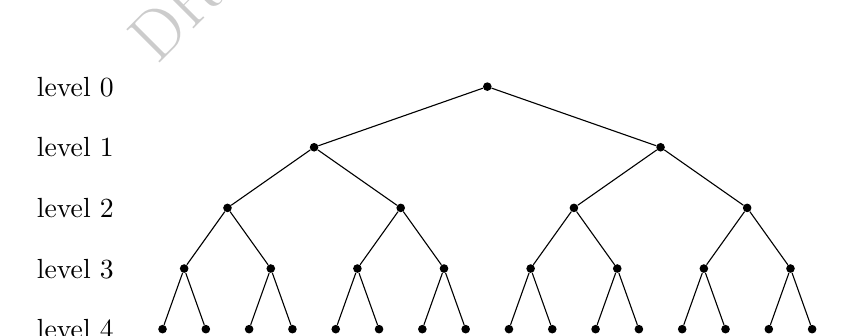
\begin{tikzpicture}[scale=0.55]
    \foreach \name/\x/\y in {
      r/0/0,
      a/-4/-1.4,b/4/-1.4,
      c/-6/-2.8,d/-2/-2.8,e/2/-2.8,f/6/-2.8,
      g/-7/-4.2,h/-5/-4.2,i/-3/-4.2,j/-1/-4.2,k/1/-4.2,l/3/-4.2,m/5/-4.2,n/7/-4.2,
      o/-7.5/-5.6,p/-6.5/-5.6,q/-5.5/-5.6,s/-4.5/-5.6,t/-3.5/-5.6,u/-2.5/-5.6,v/-1.5/-5.6,w/-0.5/-5.6,
      x/0.5/-5.6,y/1.5/-5.6,z/2.5/-5.6,aa/3.5/-5.6,ab/4.5/-5.6,ac/5.5/-5.6,ad/6.5/-5.6,ae/7.5/-5.6}
    {
      \node[smallv] (\name) at (\x,\y) {};
    }

    \draw (r)--(a) (r)--(b);

    \draw (a)--(c) (a)--(d);
    \draw (b)--(e) (b)--(f);

    \draw (c)--(g) (c)--(h);
    \draw (d)--(i) (d)--(j);
    \draw (e)--(k) (e)--(l);
    \draw (f)--(m) (f)--(n);

    \draw (g)--(o) (g)--(p);
    \draw (h)--(q) (h)--(s);
    \draw (i)--(t) (i)--(u);
    \draw (j)--(v) (j)--(w);
    \draw (k)--(x) (k)--(y);
    \draw (l)--(z) (l)--(aa);
    \draw (m)--(ab) (m)--(ac);
    \draw (n)--(ad) (n)--(ae);

    \node[left] at (-8.4,0) {level $0$};
    \node[left] at (-8.4,-1.4) {level $1$};
    \node[left] at (-8.4,-2.8) {level $2$};
    \node[left] at (-8.4,-4.2) {level $3$};
    \node[left] at (-8.4,-5.6) {level $4$};
  \end{tikzpicture}
  \end{center}

  \item At level $k$, a complete binary tree has
  \[
    2^k
  \]
  vertices. Therefore the total number of vertices from level $0$ to level $h$ is
  \[
    2^0+2^1+2^2+\cdots+2^h.
  \]
  This is a finite geometric series:
  \[
    2^0+2^1+\cdots+2^h
    =
    \frac{2^{h+1}-1}{2-1}
    =
    2^{h+1}-1.
  \]
  The leaves are exactly the vertices at level $h$, so the number of leaves is
  \[
    2^h.
  \]
  Hence
  \[
    \boxed{\text{vertices }=2^{h+1}-1,\qquad \text{leaves }=2^h.}
  \]
\end{enumerate}

\subsubsection{Method 2: Recursive recurrence}
Let
\[
  V_h=\text{number of vertices in a complete binary tree of height }h,
\]
and
\[
  L_h=\text{number of leaves in a complete binary tree of height }h.
\]

For $h=0$, the tree consists of a single root, so
\[
  V_0=1,
  \qquad
  L_0=1.
\]

For $h\ge 1$, the root has two complete binary subtrees of height $h-1$. Therefore
\[
  V_h=1+2V_{h-1},
  \qquad
  L_h=2L_{h-1}.
\]
Solving the leaf recurrence gives
\[
  L_h=2^hL_0=2^h.
\]
Solving the vertex recurrence gives
\[
  V_h=1+2+2^2+\cdots+2^h=2^{h+1}-1.
\]
Thus a complete binary tree of height $h$ has
\[
  \boxed{2^{h+1}-1\text{ vertices and }2^h\text{ leaves}.}
\]

\end{document}
